Der experimentelle Aufbau fordert, dass die Ausleseelektronik für den Ionisationskanal einen sehr kleine Ladung in form eines sehr kleinen und kurzen Strom verstärkt welcher im Kryostaten bei $\sim\SI{20}{\milli\kelvin}$ entsteht.
Damit dieser digitalisiert werden kann ist ein Impedanzwandler notwendig um die Quelle nicht zu belasten.
Dazu werden in der Regel Ladungsverstärker verwendet\cite{Censier2012}.
Diese wandeln ein Ladungsmenge in eine dazu proportionales Spannungssignal um.

Durch die Verwendung von HEMTs ist eine komplette Kryogene Verstärkerelektronik bei $\SI{4}{\kelvin}$ möglich.
Diese hat den Vorteil des niedrigen Rauschen der HEMTs sowie ihr geringer Leistungsverbrauch.
Zusätzlich kann das Signal in unmittelbar nähe zum Detektor ausgelesen werden.
Dadurch ist das Signal weniger anfällig für Störungen durch die langen Kabel aus dem Kryostaten heraus.

Das Schaltbild der Ausleseelektronik ist in Abbildung \ref{fig:Ausleseelektronik} dargestellt und ist eine Form eines Ladungsverstärkers.
Bei einem Event entsteht eine bestimmte Anzahl von Elektron-Loch-Paaren abhängig von der deponierten Energie und dem Detektormaterial.
Bei Germanium Kristallen entsteht ein Elektron-Loch-Paar pro $\sim\SI{3}{\electronvolt}$ deponierter Energie.

\begin{figure}[!t]
\begin{center}
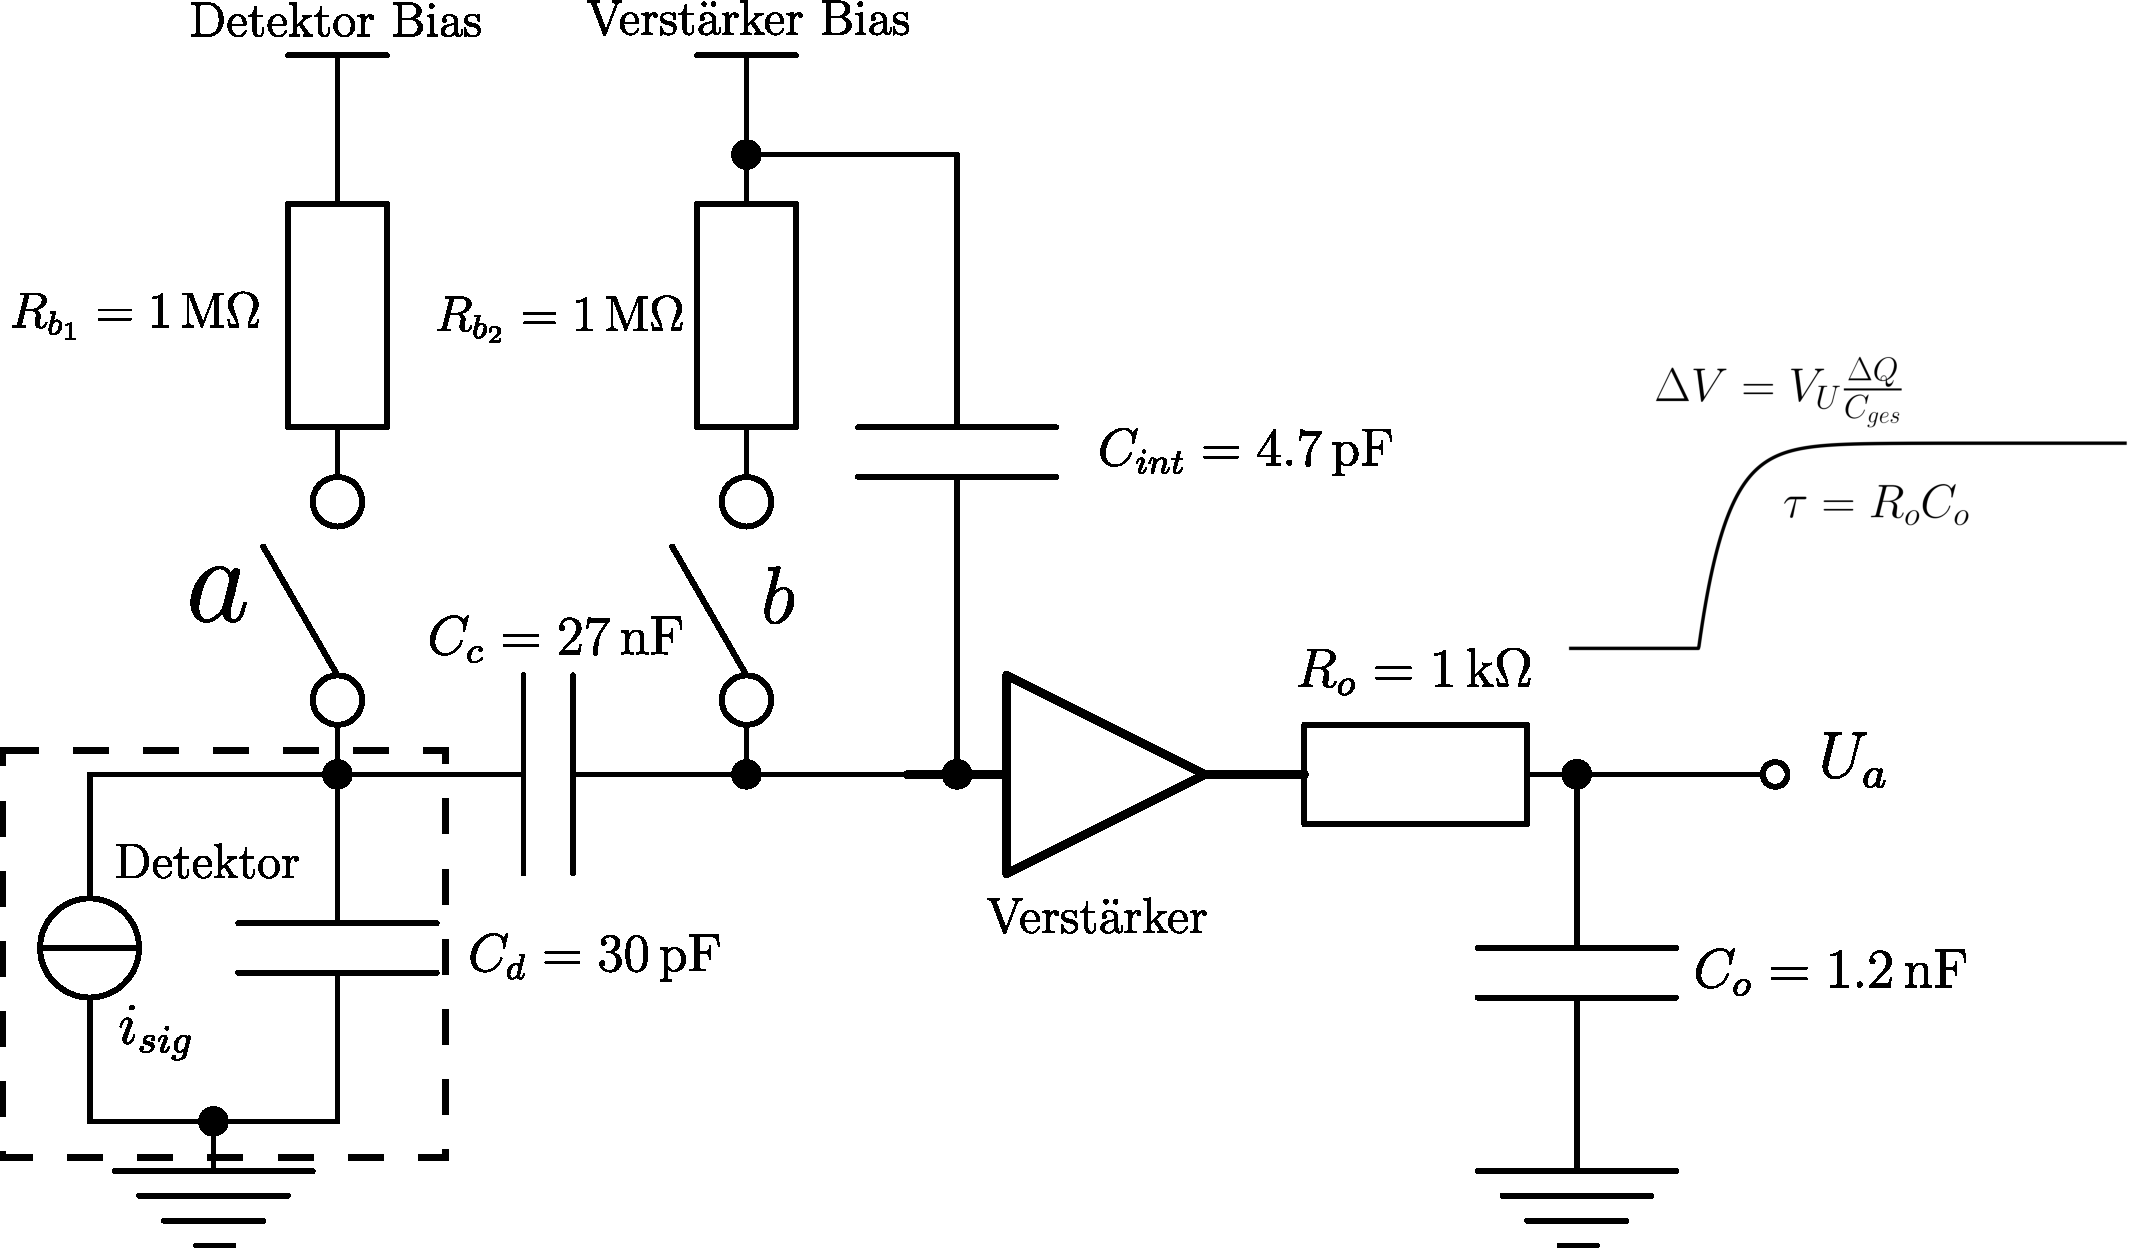
\includegraphics[width=\textwidth]{./fig/Ausleseelektronik.pdf}
\vspace{-0.5cm}
\caption{Das Design der Kalte Elektronik entspricht dem eines Ladungsverstärkers.
Der Detektor ist durch sein Ersatzschaltbild entsprechend dem Ramo-Theorem als Stromquelle parallel zur Detektorkapazität dargestellt.
Der Verstärker ist vereinfacht als Dreieck dargestellt.
Nicht eingezeichnet ist die Versorgungsspannung des Verstärkers und die Spannung zum schalten der Relais.}
\label{fig:Ausleseelektronik}
\end{center}
\end{figure}

Der Detektor wird entsprechend dem Ramo-Theorem im Ersatzschaltbild durch eine Stromquelle parallel zur Detektorkapazität dargestellt.
Der Signalstrom ist nach Gleichung \eqref{eq:RamoCurrent} abhängig von der Driftgeschwindigkeit.
In Germanium beträgt diese abhängig von der angelegten Biasspannung mehrere $\SI{}{\centi\meter}/\SI{}{\micro\second}$\cite{Jacoboni1981}.
Um in einem $\sim\SI{2}{\centi\meter}$ dicken Detektor den genauen Stromverlauf zu verfolgen ist somit ein Verstärker mit einer Bandbreite von mehreren $\SI{}{\mega\hertz}$ notwendig.
Der genaue Verlauf ist allerdings für Energiebestimmung uninteressant.
Weshalb wir uns auf den Bereich zwischen $DC\--\SI{100}{\kilo\hertz}$ beschränken.
Daher wird der Signalstrom als Deltapeak modelliert werden
\begin{equation}
i_{sig}(t) = \Delta Q \delta(t) = -eN_{eh}(a-b)\delta(t).
\end{equation}
$\Delta Q$ ist die Ladung welche gemäß dem Ramo-Theorem Gleichung \eqref{eq:RamoCharge} in der Elektrode induziert wird.

Um den kurzen Signalstrom zu messen wird dieser auf den zur Stromquelle parallelen Kapazität integriert.
Sodass ein stufenförmiges Spannungssignal entsteht.

Die Schalter dienen dazu die Kapazitäten vor zu spannen damit am Detektor und am Eingang des Verstärkers die gewünschten Biasspannungen anliegen.
Im Normalbetrieb sind die Schalter offen.
Dies hat den Vorteil, dass das Rauschen der Spannungsquellen und der Biaswiderstände nicht das Signal verunreinigen.

Da der Detektor und der Verstärkereingang in der Regel auf unterschiedlichen DC Level liegen ist die Koppelkapazität $C_c$ notwendig.
Da die Kapazität $C_c$ das Signal allerdings wider differenziert ist eine weitere Kapazität $C_int$ notwendig welche das Signal am Eingang des Verstärkers integriert.
Die Koppelkapazität belastet das Signal gemäß
\begin{equation}
\frac{U_e}{U_s} = \frac{C_c}{C_c + C_{int}} \stackrel{C_{int} \ll C_c}{\approx} 1.
\end{equation}
Das heißt die Koppeleffizienz geht gegen $1$ wenn die Koppelkapazität deutlich größer gewählt wird als die Kapazität $C_{int}$.

Die Fouriertransformation des Signalstroms ist $i_{sig}(f)=\Delta Q$.
Durch Multiplikation mit der Eingangsimpedanz bei geschlossenen Schalter $a$ und offenem Schalter $b$ erhalten wir das Spannungssignal
\begin{equation}
U_{sig}(f) = i_{sig}(f)Z_{ein} = i_{sig}(R_b||Z_{C_{ges}}) = \Delta Q \frac{R_b}{1 + j2\pi f C_{ges}R_b}.
\label{eq:InitialSig}
\end{equation}
Die Kapazität $C_{ges}$ ist die Gesamtkapazität aus der Detektorkapazität $C_d$, der Koppelkapazität $C_c$, und der Kapazität $C_{int}$ 
\begin{equation}
C_{ges} = C_d + \frac{C_cC_{int}}{C_{int} + C_c} \stackrel{C_{int} \ll C_c}{\approx} C_d + C_{int}.
\end{equation}
Im Zeitraum erhalten wir dann für das Spannungssignal
\begin{equation}
U_{sig}(t) = \frac{\Delta Q}{C_{ges}}e^{-\frac{t}{R_bC_{ges}}}\Theta(t).
\end{equation}
Wie erwartet kommt es also zu einem Sprung dessen Höhe $\Delta Q/C_{ges}$ die relevante Information über die Anzahl der Ladungsträger und damit der deponierten Energie enthält.
Die Stufe fällt allerdings mit der Zeitkonstante $\tau=R_bC_{ges}$ exponentiell ab.
Im normalen betrieb ist jedoch auch der Schalter $a$ geöffnet.
Dies entspricht $R_b\rightarrow\inf$ das heißt
\begin{equation}
U_{sig}(t)\rightarrow U_{sig}(t)=\frac{\Delta Q}{C_{ges}}\Theta(t).
\end{equation}
Da die Stufe somit nicht mehr abklingt ist es notwendig das DC Level in bestimmten Zeitintervallen durch schließen der Schalter zurückzusetzen.

Durch einen Tiefpass am Ausgang des Verstärkers wird das Frequenzband auf den interessanten Bereich $DC \-- \SI{100}{\kilo\hertz}$ eingeschränkt.
Dies verbessert das Signal zu Rausch Verhältnis und verhindert gleichzeitig, dass hochfrequente Schwingungen über die langen Kabel auf den Eingang des Verstärkers Rückkoppeln wodurch der Verstärker anfangen kann zu oszillieren.
Die Grenzfrequenz ist gegeben durch 
\begin{equation}
f_{-3\,\mathrm{db}} = \frac{1}{2\pi R_o C_o}
\end{equation}

Die Form des Signals nach dem Verstärker und dem Tiefpass lässt sich am einfachsten bestimmen wenn wir wieder von Gleichung \eqref{eq:InitialSig} ausgehen und zum Schluss  den Widerstand $R_b$ gegen unendlich gehen lassen um das verhalten bei offenem Schalter zu erhalten.
Indem wir also Gleichung \eqref{eq:InitialSig} mit der Übertragungsfunktion des Verstärkers $\alpha(f)$ und des Tiefpass multiplizieren erhalten wir
\begin{equation}
U_{sig}(f) = \Delta Q \frac{R_b}{1 + j2\pi f C_{ges}R_b} \alpha(f) \frac{1}{1 + j 2 \pi f C_o R_o}.
\end{equation}
Der Verstärker verhält sich auch wie ein Tiefpass dessen Grenzfrequenz allerdings deutlich größer ist.
Daher kann die Übertrangungsfunktion des Verstärkers als konstant angenommen werden $\alpha(f) = V_U$ in dem von uns betrachteten Frequenzband.
Durch die Rücktransformation erhalten wir schließlich
\begin{equation}
U_{sig}(t) = V_U \frac{\Delta Q}{C_{ges}}(1 - e^{-t/R_oC_o}).
\end{equation}
In der Abbildung \ref{fig:Ausleseelektronik} ist die Form des Ausgangssignals rechts im Bild dargestellt.
